\documentclass{standalone}

\usepackage{tikz}
\usetikzlibrary{positioning}

\newcommand{\JustifiedLine}[2][1]{\resizebox{#1\linewidth}{!}{#2}}

\usepackage{xcolor}
\definecolor{bggreen}{HTML}{40B9B2}
\definecolor{lightgreen}{HTML}{7CCCBF}
\definecolor{hotblue}{HTML}{1D255C}
\definecolor{titleblue}{HTML}{043340}

\usepackage{fontspec}
\newfontfamily{\authorfont}{Alber}
\newfontfamily{\titlefont}{PT Serif}

\usepackage{anyfontsize}
\def\titleset{\fontsize{60}{0}\selectfont\titlefont}
\def\authorset{\fontsize{35}{0}\selectfont\authorfont}
\def\lmsset{\fontsize{30}{0}\selectfont\authorfont}

\begin{document}
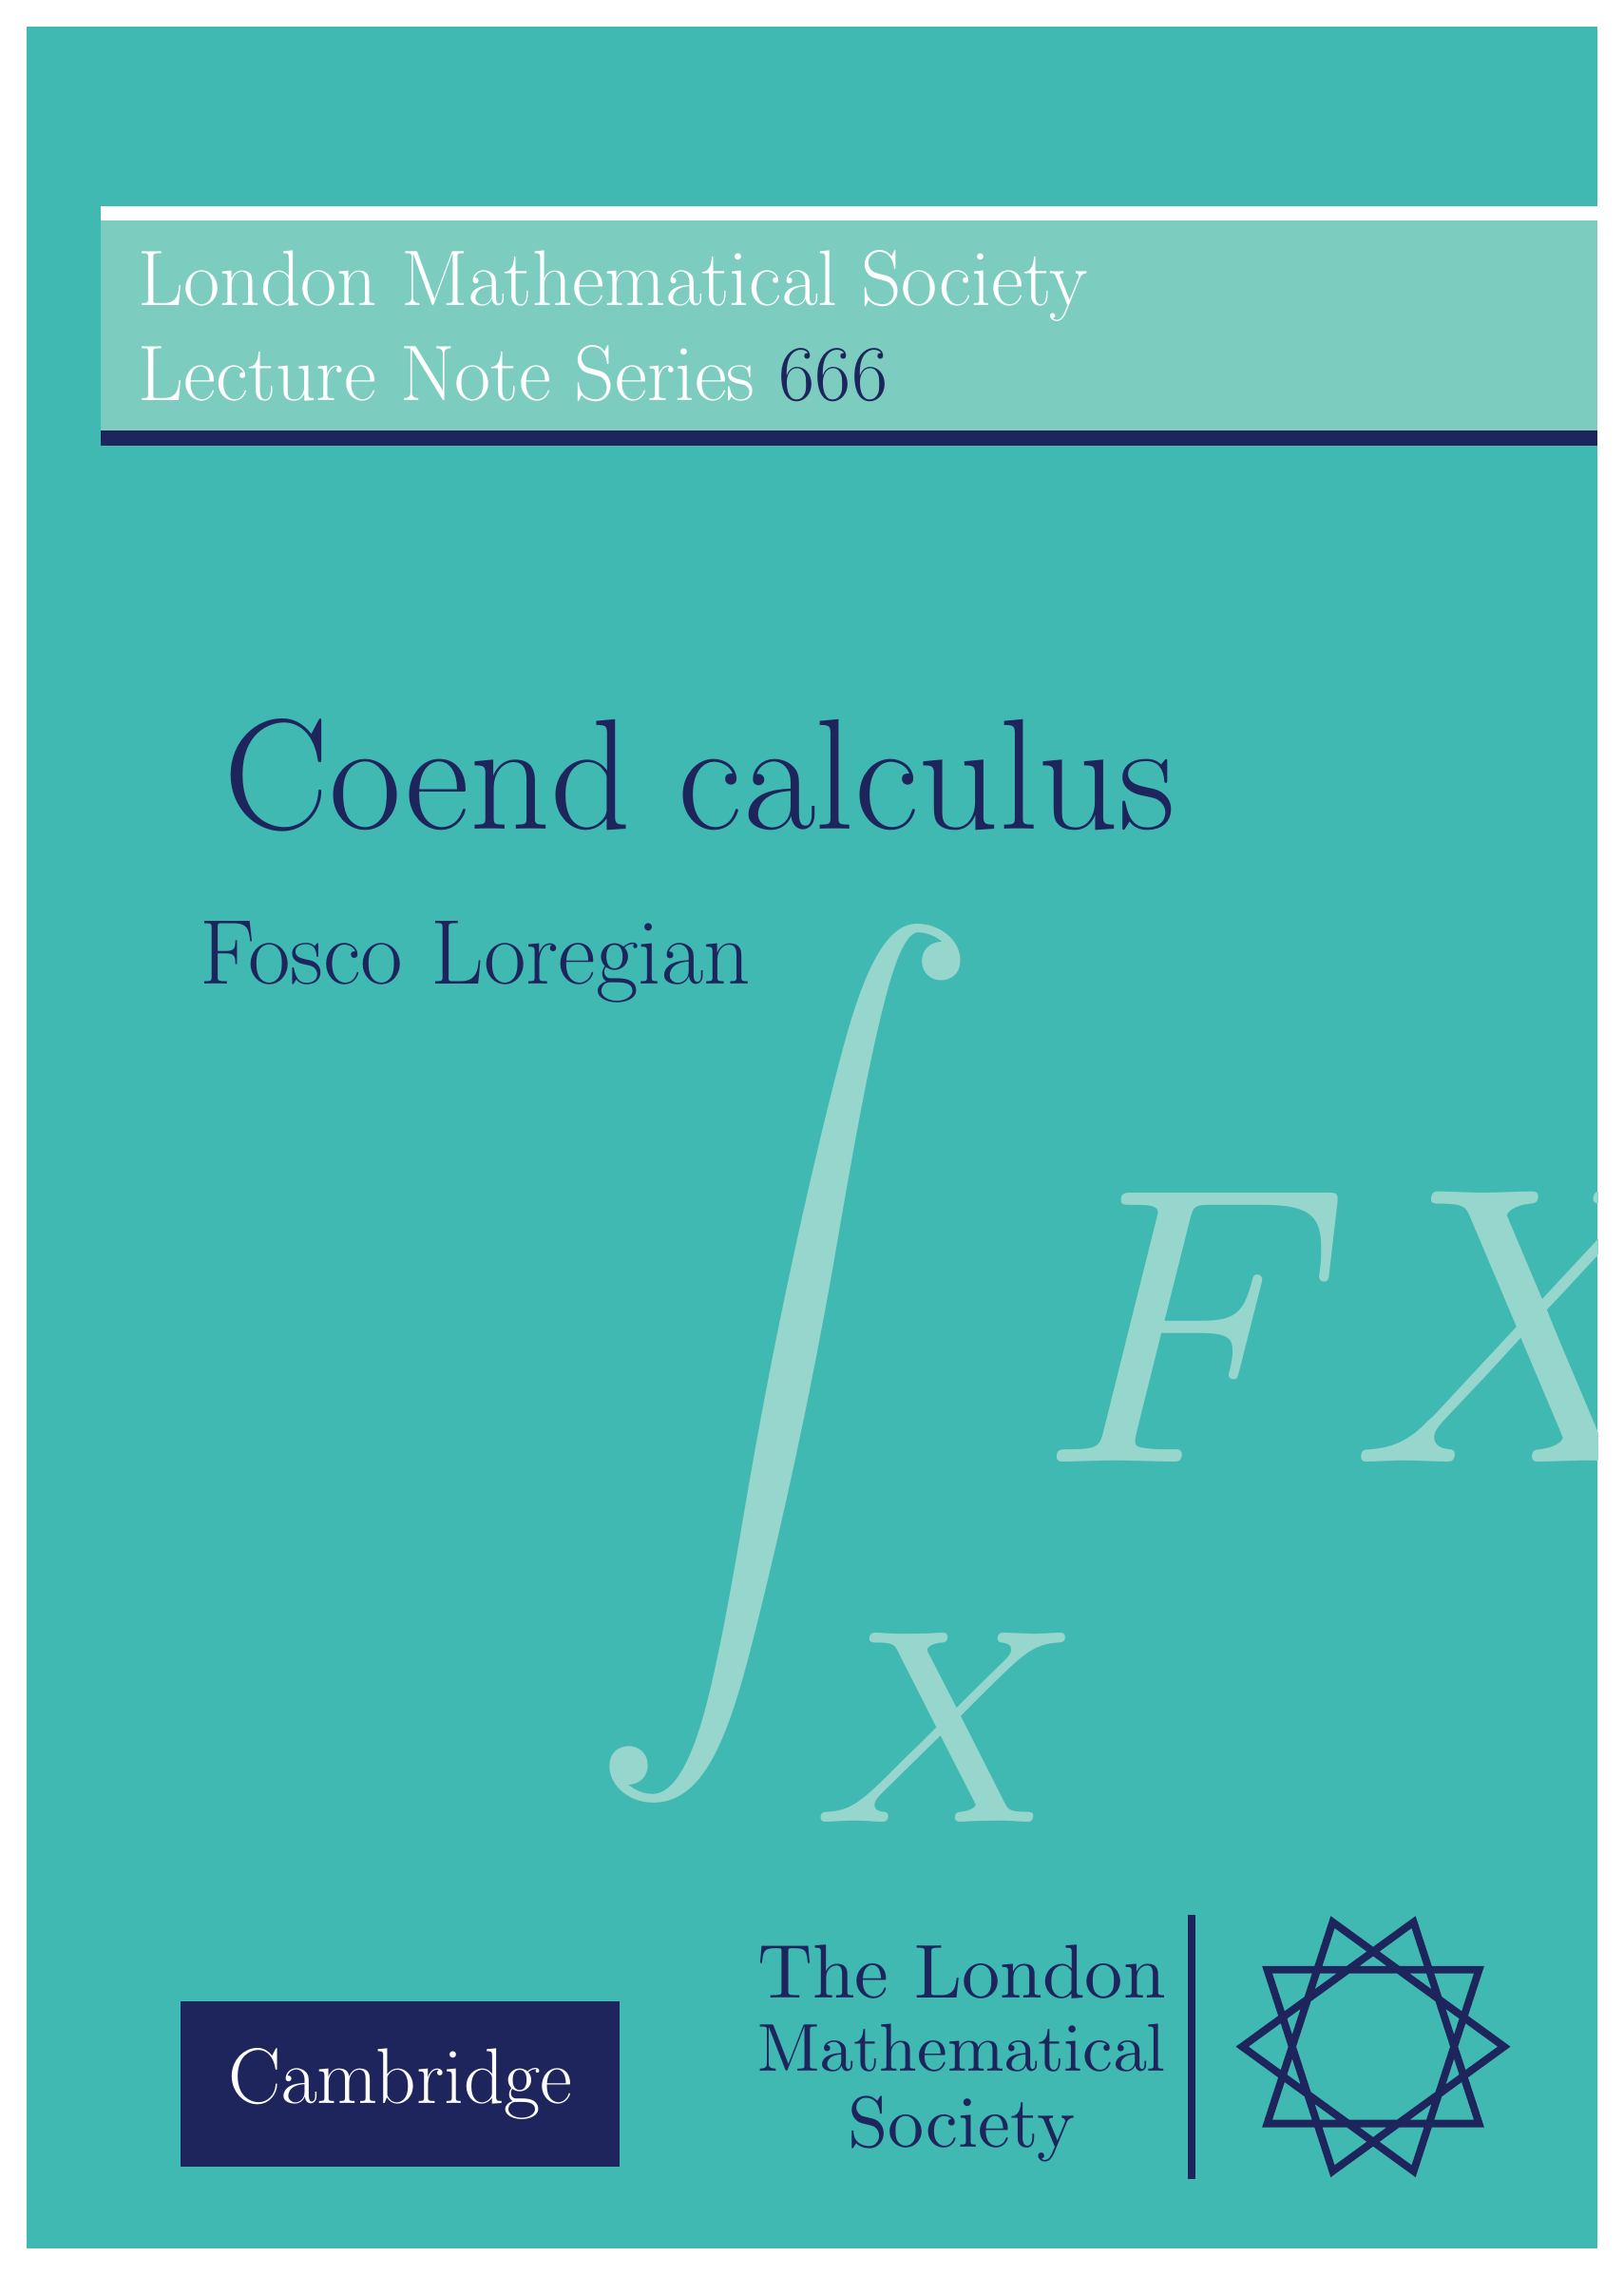
\begin{tikzpicture}[yscale=-1]
% contour
\clip (0,0) rectangle (210mm,297mm);

\fill[bggreen] (0,0) rectangle (210mm,297mm);
\node[white!20!lightgreen] at (150mm,180mm)
  {\resizebox{15cm}{!}{$\displaystyle\int_X\!\! FX$}};
\node[hotblue] (title) at (9,100mm)
  {\titleset Coend calculus};
\node[hotblue] (author) at (6,125mm)
  {\authorset Fosco Loregian};

\foreach \i in {0,...,9}
  \coordinate[yshift = -270mm, xshift=18cm] (\i) at (\i*36:1.75);

\draw[hotblue, line width=1mm] (0)
  -- (3)
  -- (6)
  -- (9)
  -- (2)
  -- (5)
  -- (8)
  -- (1)
  -- (4)
  -- (7)
  -- cycle;
\fill[lightgreen] (1,2.5) rectangle (210mm,5.5);
\draw[white, line width=2mm]
  (210mm,2.5) -- (1,2.5) node[below right=4mm]
  {\lmsset London Mathematical Society};
\draw[hotblue, line width=2mm]
  (210mm,5.5) -- (1,5.5) node[above right=4mm]
  {\lmsset \textcolor{white}{Lecture Note Series} \textcolor{hotblue}{666}};

\node[inner sep=18pt,fill,ultra thick, hotblue] at (5,275mm)
  {\Huge \textcolor{white}{\titlefont Cambridge}};

\coordinate[yshift = -270mm, xshift=18cm] (A1) at (4*36:3);
\coordinate[yshift = -270mm, xshift=18cm] (A2) at (6*36:3);
\draw[line width=1mm, hotblue] (A1) -- (A2);

\begin{scope}[yshift=260mm, xshift=12.5cm, hotblue]
\node (thelondon) at (0,0)
  {\JustifiedLine[.45]{\authorfont The London}};
\node[below=1mm of thelondon] (math)
  {\JustifiedLine[.45]{\authorfont Mathematical}};
\node[below=1mm of math] (soc)
  {\JustifiedLine[.25]{\authorfont Society}};
\end{scope}

\end{tikzpicture}
\end{document}
